\documentclass[10pt, aspectratio=169]{beamer}
\usepackage[utf8]{inputenc}
\usepackage[magyar]{babel}
\usepackage{amsmath, amsfonts}
\usepackage{bm}
\usepackage{calc}
\usepackage{newtxmath}
\usepackage{microtype}
\usepackage{mathdots}
\usepackage{mathtools}
\usepackage{siunitx}

\usepackage{tikz}
\usetikzlibrary{shapes,arrows}
\usetikzlibrary{tikzmark,positioning}
\usepackage{pgfplots}
\usepgfplotslibrary{patchplots}
% 
% \definecolor{tkpblue}{rgb}{0.0, 0.627, 0.961}
% \definecolor{tkplightblue}{rgb}{0.455, 0.769, 0.937}
% \definecolor{tkplightgrey}{rgb}{0.851, 0.871, 0.910}
% \definecolor{tkpdarkgrey}{rgb}{0.3, 0.3, 0.35}     % for subtle lines or labels
% \definecolor{tkptext}{rgb}{0.294, 0.333, 0.392}
% \definecolor{tkphighlight}{rgb}{0.9, 0.5, 0.2}
% \definecolor{tkpgreen}{rgb}{0.2, 0.65, 0.35}    % fresh green
% \definecolor{tkpteal}{rgb}{0.0, 0.6, 0.6}       % balanced teal
% \definecolor{tkppurple}{rgb}{0.5, 0.3, 0.7}     % gentle violet
% \definecolor{tkpyellow}{rgb}{0.95, 0.75, 0.1}   % rich yellow
% \definecolor{tkplightyellow}{rgb}{1.0, 0.95, 0.75}
% \definecolor{tkpred}{rgb}{0.85, 0.2, 0.2}       % vivid red
% \definecolor{tkpbrown}{rgb}{0.6, 0.4, 0.2}      % earthy brown
% \definecolor{tkpmidgrey}{rgb}{0.6, 0.6, 0.7}       % for background reference

\definecolor{rd}{RGB}{178,34,34}
\definecolor{rd2}{RGB}{230,0,0}
\definecolor{gr}{RGB}{107,142,35}
\definecolor{gr2}{RGB}{0,209,0}
\definecolor{bl}{rgb}{0.0, 0.627, 0.961}
\definecolor{grey}{rgb}{0.651, 0.671, 0.710}
\definecolor{or}{RGB}{255,128,0}


% \pgfplotscreateplotcyclelist{tkpcolors}{
%   {color=tkpblue},
%   {color=tkpbrown},
%   {color=tkpred},
%   {color=tkpgreen},
%   {color=tkppurple},
%   {color=tkpteal}
% }
% 
% \pgfplotsset{
%   every axis/.append style={
%     cycle list name=tkpcolors
%   }
% }
% 
% \pgfplotsset{
%     colormap/tkpbluebrown/.style={
%         colormap={tkpbluebrown}{
%             rgb=(0.0, 0.627, 0.961)   % tkpblue
%             rgb=(0.9, 0.5, 0.2)      % tkphighlight (bridge color)
%             rgb=(0.6, 0.4, 0.2)      % tkpbrown
%         }
%     }
% }
% 
% 
% \pgfplotsset{
%     colormap/tkpbluegreen/.style={
%         colormap={tkpbluegreen}{
%             rgb=(0.0, 0.627, 0.961)    % tkpblue
%             rgb=(0.0, 0.6, 0.6)        % tkpteal
%             rgb=(0.2, 0.65, 0.35)      % tkpgreen
%             rgb=(0.95, 0.75, 0.1)      % tkpyellow
%             rgb=(0.9, 0.5, 0.2)        % tkphighlight
%         }
%     }
% }

\definecolor{PGreen}{HTML}{CDECCB}
\definecolor{POrange}{HTML}{FFE2C2}
\definecolor{PBlue}{HTML}{5E8CCB}
\definecolor{Charcoal}{HTML}{1F1F1F}

% Extra complementary colors:
\definecolor{PLightBrown}{HTML}{D6BFA3}  
\definecolor{PMedBrown}{HTML}{A67855}  
\definecolor{PDarkBrown}{HTML}{4B2E1E}

\definecolor{PLightBlue}{HTML}{B8D9EB}% light sky blue
\definecolor{PLightGray}{HTML}{E6E6E6} % for subtle backgrounds
\definecolor{PPurple}{HTML}{C4B4D9}     % muted pastel purple
\definecolor{PYellow}{HTML}{F9EBA5}     % slightly darker pastel yellow
\definecolor{PMauve}{HTML}{BFA1C8}  % pasztell lila
\usetheme[progressbar=none, numbering=fraction, titleformat=smallcaps]{metropolis}           % Use metropolis theme
\setbeamercolor{progress bar}{fg=PBlue}
\setbeamercolor{progress bar in head/foot}{fg=PBlue}
\setbeamercolor{progress bar in section page}{fg=PBlue}




\setbeamercolor{normal text}{fg=Charcoal,bg=white}
\setbeamercolor{structure}{fg=PBlue}

% Headline & titles
\setbeamercolor{title}{fg=PBlue!60!black}
\setbeamercolor{frametitle}{fg=white,bg=PBlue}
\setbeamercolor{titlelike}{fg=PBlue!60!black}
\setbeamercolor{title separator}{fg=PBlue}

% Blocks
\setbeamercolor{block title}{fg=Charcoal,bg=PLightGray!80}
\setbeamercolor{block body}{fg=Charcoal,bg=PLightGray!30}

\setbeamercolor{alerted text}{fg=POrange!70!red}

\setbeamercolor{block title alerted}{fg=Charcoal,bg=POrange}
\setbeamercolor{block body alerted}{fg=Charcoal,bg=POrange!50}
% 

% ---------- Section-szerinti számláló ----------
\newcounter{thm}[section]
\renewcommand{\thethm}{\thesection.\arabic{thm}}

% ---------- Saját theorem környezet ----------
\newenvironment{blockthm}[1][]{%
  \refstepcounter{thm}%
  \setbeamercolor{block title}{fg=Charcoal,bg=PLightBlue!80}%
  \setbeamercolor{block body}{fg=Charcoal,bg=PLightBlue!30}%
  \begin{block}{\thethm. Tétel#1}%
}{%
  \end{block}%
}

% ---------- Saját definition környezet ----------
\newenvironment{blockdef}[1][]{%
  \refstepcounter{thm}%
  \setbeamercolor{block title}{fg=Charcoal,bg=PYellow!80}%
  \setbeamercolor{block body}{fg=Charcoal,bg=PYellow!30}%
  \begin{block}{\thethm. Definíció#1}%
}{%
  \end{block}%
}

% ---------- Saját lemma környezet ----------
\newenvironment{blocklem}[1][]{%
  \refstepcounter{thm}%
  \setbeamercolor{block title}{fg=Charcoal,bg=PPurple!80}%
  \setbeamercolor{block body}{fg=Charcoal,bg=PPurple!30}%
  \begin{block}{\thethm. Lemma#1}%
}{%
  \end{block}%
}


% ---------- Saját lemma környezet ----------
\newenvironment{exercise}[1][]{%
  \refstepcounter{thm}%
  \setbeamercolor{block title}{fg=Charcoal,bg=PGreen!80}%
  \setbeamercolor{block body}{fg=Charcoal,bg=PGreen!30}%
  \begin{block}{\thethm. Feladat#1}%
}{%
  \end{block}%
}

\newcommand{\R}{\mathbb{R}}
\newcommand{\Z}{\mathbf{Z}}
\DeclareMathOperator*{\argmin}{arg\,min}
\DeclareMathOperator{\diag}{diag}
\DeclareMathOperator{\sat}{sat}
\DeclareMathOperator{\var}{Var}

\DeclareMathOperator{\dom}{dom}

\newcommand{\bx}{\mathbf{x}}
\newcommand{\ba}{\mathbf{a}}
\newcommand{\bhx}{\mathbf{\hat{x}}}
\newcommand{\by}{\mathbf{y}}
\newcommand{\bhy}{\mathbf{\hat{y}}}
\newcommand{\bu}{\mathbf{u}}
\newcommand{\bb}{\mathbf{b}}
\newcommand{\bF}{\mathbf{F}}
\newcommand{\bp}{\mathbf{p}}
\newcommand{\bd}{\mathbf{d}}
\newcommand{\bq}{\mathbf{q}}


\newcommand{\bA}{\mathbf{A}}
\newcommand{\bC}{\mathbf{C}}
\newcommand{\bX}{\mathbf{X}}
\newcommand{\bM}{\mathbf{M}}
\newcommand{\bH}{\mathbf{H}}
\newcommand{\bS}{\mathbf{S}}
\newcommand{\bI}{\mathbf{I}}
\newcommand{\bR}{\mathbf{R}}
\newcommand{\bQ}{\mathbf{Q}}


\newcommand{\bbeta}{\boldsymbol{\beta}}
\newcommand{\beps}{\boldsymbol{\epsilon}}
\newcommand{\bnu}{\boldsymbol{\nu}}
\newcommand{\blambda}{\boldsymbol{\lambda}}
\newcommand{\bSigma}{\boldsymbol{\Sigma}}


% % \renewtheorem{theorem}{Tétel}[section]
% \newtheorem{lemma}[theorem]{Lemma}
% \newtheorem{definition}[theorem]{Definíció}


\newcommand{\hl}[2][tkplightyellow]{\mathchoice%
 {\colorbox{#1}{$\displaystyle#2$}}%
 {\colorbox{#1}{$\textstyle#2$}}%
 {\colorbox{#1}{$\scriptstyle#2$}}%
 {\colorbox{#1}{$\scriptscriptstyle#2$}}}%


% \usefonttheme[onlymath]{serif}
\usepackage[sfdefault, lining]{FiraSans}
\renewcommand*\oldstylenums[1]{{\firaoldstyle #1}}


\renewcommand{\emph}[1]{{\bf #1}}


\newcommand{\nb}[2]{(#1)_{#2}}
\newcommand{\D}{\mathbb{D}}
\newcommand{\N}{\mathbb{N}}



\title{A Gausz-függvény univerzalitása}
\date{\today}
\author{Csikja Rudolf}

\begin{document}
\begin{frame}{}
\titlepage
\end{frame}

\begin{frame}{}
\tableofcontents
\end{frame}


\section{Bevezetés}
\begin{frame}[t]{A harang görbe jelentősége}

\begin{columns}
\begin{column}{0.4\textwidth}
\begin{center}
\includegraphics[scale=0.08]{Carl_Friedrich_Gauss_1840.jpg}\\
Carl Friedrich Gauss (1777--1855) 
\end{center}


\end{column}
\begin{column}{0.6\textwidth}
Johann Carl Friedrich Gauss német matematikus, csillagász, geodéta és fizikus.
\end{column}
 
\end{columns}
\end{frame}

\section{A Gauss függvény elemi vizsgálata}

\subsection{Alapvető tulajdonságok}
\begin{frame}{Definíció}
 \begin{columns}
\begin{column}{0.45\textwidth}

\begin{blockdef}[~ (Gauss függvény)]
A valós $g\colon \R \to \R$ függvényt
\[g(x) := \exp\left(-\frac{x^2}{2}\right)\]
(standard) Gauss függvénynek hívjuk.
\end{blockdef}
\end{column}
\begin{column}{0.45\textwidth}
 \pgfplotsset{width=\columnwidth,compat=1.9}
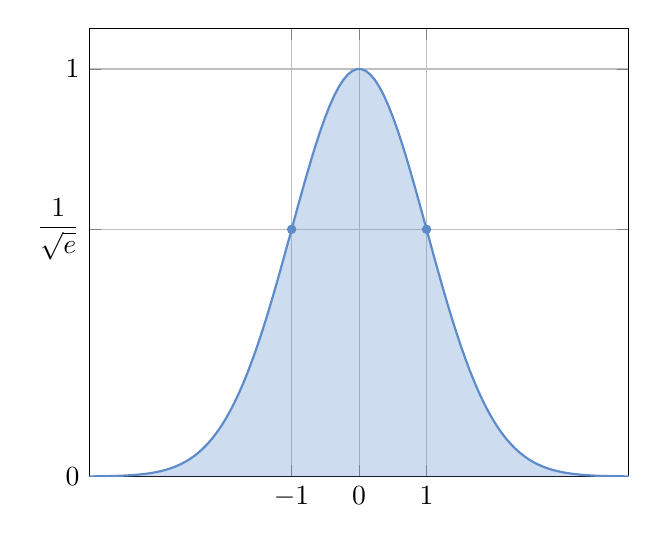
\begin{tikzpicture}[scale=1]
    \begin{axis}[
        xmin = -4, xmax = 4,
        ymin = -0.0, ymax = 1.1,
        mark=none,
        xtick={-1,0,1},
        ytick={0,{1/sqrt(e)}, 1},
        xticklabels={$-1$,$0$,$1$},
        yticklabels={$0$,$\dfrac{1}{\sqrt e}$,$1$},
        grid=major,
        minor tick num=0,
    ]
    \addplot[color=PBlue, fill=PBlue, fill opacity=0.3, domain=-5:5, thick, samples=150]{exp(-(x^2/2))};
    \addplot[
        only marks,
        mark=*,
        mark size=1.5pt,
        color=PBlue] 
            coordinates {
            (-1,{1/sqrt(e)})
            (1,{1/sqrt(e)})
            };
    \end{axis}
    
\end{tikzpicture}

\end{column}
 
\end{columns}
\end{frame}


\begin{frame}{Alapvető tulajdonságok}
A következő tételben a Gauss függvény néhány alapvető tulajdonságát fogalmazzuk meg.
\begin{blockthm}
A Gauss függvény az alábbi tulajdonságokkal rendelkezik:
\begin{enumerate}[a)]
 \item Minden $x\in\R$ esetén $g(x) > 0$.
 \item Globális maximuma van az $x=0$ pontban, és monoton növekvő a $(-\infty, 0),$ illetve monoton csökkenő a $(0, +\infty)$ intervallumon.
 \item Inflexiós pontja van az $x=1$ és $x=-1$ pontokban, továbbá konkáv a $(-\infty, -1)$ és az $(1, +\infty)$ intervallumokon, illetve konvex a $(-1, 1)$ intervallumon.
\end{enumerate}
\end{blockthm}

\begin{exercise}
 Bizonyítsuk be a fenti tételt!
\end{exercise}

\end{frame}


\begin{frame}[t]{Általános Gauss-függvények}
\[G_{\mu,\sigma}(x) := g\left(\frac{x-\mu}{\sigma}\right), \qquad g(x) = G_{\mu,\sigma}(\sigma(x+\mu))\] 
\end{frame}




\begin{frame}[t]{A cos függvény hatványai}
\begin{columns}
\begin{column}{0.4\textwidth}
\[f_n(x):=\cos^n(x), \quad x\in(-\pi/2, \pi/2)\] 
\begin{center}
\pgfplotsset{width=\columnwidth,compat=1.9}
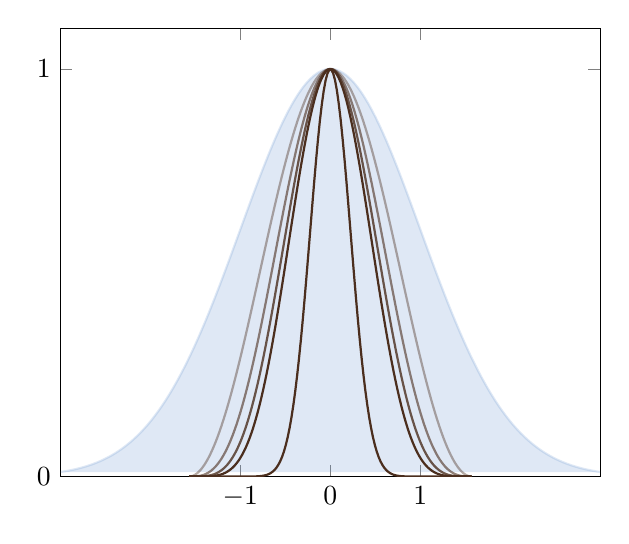
\begin{tikzpicture}[scale=1]
    \begin{axis}[
        trig format plots=rad,
        xmin = -3, xmax = 3,
        ymin = -0.0, ymax = 1.1,
        mark=none,
        xtick={-1,0,1},
        ytick={0, 1},
        xticklabels={$-1$,$0$,$1$},
        yticklabels={$0$,$1$}
    ]
    \addplot[color=PBlue, fill=PBlue, opacity=0.2, domain=-3:3, thick, samples=150]{exp(-(x^2/2))};
    \addplot[color=PDarkBrown, opacity=0.4, domain=-1.57:1.57, thick, samples=150]{cos(x)^2};
    \addplot[color=PDarkBrown, opacity=0.6, domain=-1.57:1.57, thick, samples=150]{cos(x)^3};
    \addplot[color=PDarkBrown, opacity=0.8, domain=-1.57:1.57, thick, samples=150]{cos(x)^4};
    \addplot[color=PDarkBrown, opacity=1.0, domain=-1.57:1.57, thick, samples=150]{cos(x)^5};
    \addplot[color=PDarkBrown, opacity=1.0, domain=-1.57:1.57, thick, samples=150]{cos(x)^20};

    \end{axis}
    
\end{tikzpicture}

\end{center}
Az $s_n$ inflexiós pontokban
\[f_n(s_n) \to \frac{1}{\sqrt{e}}\]
\end{column}
\begin{column}{0.6\textwidth}
A probléma, hogy $s_n\to0,$ miközben a Gauss függvény inflexiós pontja $\pm1.$
A megoldás, hogy minden egyes függvényre újraskálázzuk az értelmezési tartományt úgy,
hogy az új függvénynek $\pm1$ pontban legyen az inflexiós pontja:
\[g_n(x):=f_n(s_n x) = \cos^n(s_n x), \quad  -\frac{\pi}{2s_n} \le x \le \frac{\pi}{2s_n}.\]
\begin{exercise}
Bizonyítsuk be, hogy
\[g_n''(1) = 0 \quad \text{és}\quad  \lim_{n\to\infty}g_n(1) = g(1) = 1/\sqrt{e}\].
\end{exercise}

\end{column}
\end{columns}

\end{frame}

\subsection{Maximummal rendelkező függvények magas hatványai}
\begin{frame}[t]{}
\begin{columns}
  \begin{column}{0.6\textwidth}
    \begin{blocklem}
      Az $f_n$ függvény pozitív inflexiós pontja
      \[s_n = \arctan\left(\frac{1}{\sqrt{n-1}}\right), \quad n\ge 2\]
    \end{blocklem}
    \begin{exercise}
     Bizonyítsuk be, hogy az $g_n$ függvények értelmezési tartománya
     tart a $(-\infty, +\infty)$ intervallumhoz.
    \end{exercise}
    \begin{exercise}
     Végezzük el az eddigi számításokat az
     \begin{enumerate}[a)]
      \item $f_n(x):=\left(1+x^2\right)^{-n},$ $x\in(-\infty, \infty)$
      \item $f_n(x):=\cosh(x)^{-n},$ $x\in(-\infty, \infty)$
     \end{enumerate}
      függvényekre.
    \end{exercise}    

  \end{column}
  
  \begin{column}{0.4\textwidth}
    \begin{alertblock}{Az átskálázott függvények}
      \[g_n(x) = \cos^n \left( \arctan\left(\frac{1}{\sqrt{n-1}}\right) x\right)\]
    \end{alertblock}
    \begin{center}
      \pgfplotsset{width=0.5\columnwidth,compat=1.9}
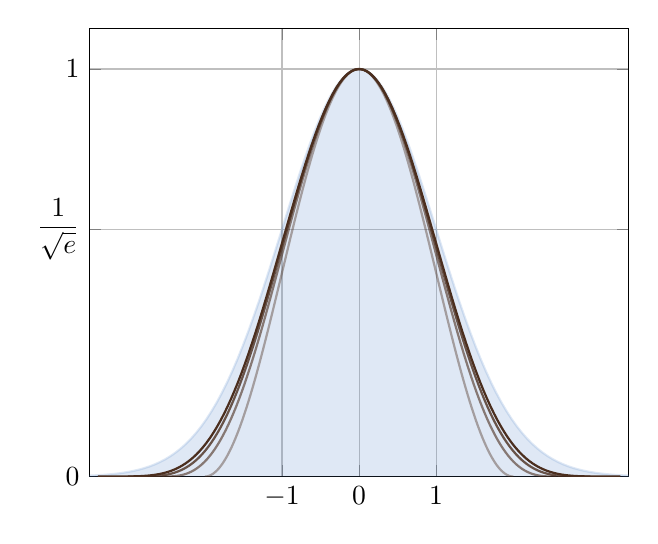
\begin{tikzpicture}[scale=1]
    \begin{axis}[
        xmin = -3.5, xmax = 3.5,
        ymin = -0.0, ymax = 1.1,
        mark=none,
        xtick={-1,0,1},
        ytick={0,{1/sqrt(e)}, 1},
        xticklabels={$-1$,$0$,$1$},
        yticklabels={$0$,$\dfrac{1}{\sqrt e}$,$1$},
        grid=major,
        minor tick num=0,
    ]
    \addplot[color=PBlue, fill=PBlue, opacity=0.2, domain=-5:5, thick, samples=150]{exp(-(x^2/2))};
    \addplot[color=PDarkBrown, opacity=0.4, domain=-2:2, thick, samples=150]{cos(x * 45)^2};
    \addplot[color=PDarkBrown, opacity=0.6, domain=-2.553:2.553, thick, samples=150]{cos(x * atan(1/sqrt(2)))^3};
    \addplot[color=PDarkBrown, opacity=0.8, domain=-3:3, thick, samples=150]{cos(x * 30)^4};
    \addplot[color=PDarkBrown, opacity=1.0, domain=-3.389:3.389, thick, samples=150]{cos(x * atan(0.5))^5};
    \end{axis}
    
\end{tikzpicture}

    \end{center}
  \end{column}
\end{columns}
\end{frame}

\begin{frame}{Univerzális konvergencia a Gauss-függvényhez}
    \begin{blockthm}{Tétel}
        Legyen $I \subseteq \mathbb{R}$ intervallum, ahol $0 \in \text{int}(I)$. Legyen $h: I \to \mathbb{R}$ olyan függvény, amelyre:
        \begin{itemize}
            \item \textbf{Maximum:} $h(0) = 1$ és $|h(x)| < 1$ minden $x \in I \setminus \{0\}$ esetén.
            \item \textbf{Simaság:} $h \in C^2$ a $0$ környezetében, $h'(0) = 0$ és $h''(0) < 0$.
        \end{itemize}
        Ekkor a $g_n(x) = h^n(s_n x)$ függvénysorozat pontonként tart a standard normális eloszlás magjához:
        \[ \lim_{n\to\infty} g_n(x) = e^{-\frac{x^2}{2}} \]
        ahol a skálázási tényező aszimptotikusan:
        \[ s_n \sim \frac{1}{\sqrt{n \cdot \frac{|h''(0)|}{2}}} \]
    \end{blockthm}
\end{frame}

\begin{frame}[t]{}
\begin{blockthm}{}
Legyen $h\colon[-a,a]\to\R^+$ egy olyan páros függvény, amelyre $h(0)=1, h'(0)=0$ és
$h''(0)<0,$ ekkor a $g_n(x) = h^n(s_n x)$ függvénysorozatra
\[\lim_{n\to\infty} g_n(x) = g(x) = e^{-\frac{x^2}{2}},\]
ahol
\[s_n = \sqrt{\frac{2}{h''(0)}} \cdot \frac{1}{\sqrt{2n-1}} = O\left(\frac{1}{\sqrt{n}}\right)\]
\end{blockthm}
\[f(s_n x) = F_n(x) = \left(1-\frac{x^2}{n}\right)^n, \quad x\in (-\sqrt{n}, \sqrt{n})\]
ami határértékben
\[F(x) = \lim_{n\to\infty} F_n(x) = \lim_{n\to\infty}\left(1-\frac{x^2}{n}\right)^n = e^{-x^2}, \quad x\in(-\infty, +\infty)\]
\end{frame}

  
  
\subsection{A Gauss fügvény integrálja}
\begin{frame}[t]{A Gauss függvény integrálja}
  \begin{blockthm}
  \[\int_{-\infty}^{+\infty} g(x)\, dx = \sqrt{\pi}\]
  \end{blockthm}
\end{frame}

\begin{frame}[t]{}
\begin{columns}
  \begin{column}{0.5\textwidth}
   
  \end{column}
  
  \begin{column}{0.5\textwidth}
 \begin{center}
    \pgfplotsset{width=0.5\columnwidth,compat=1.9}
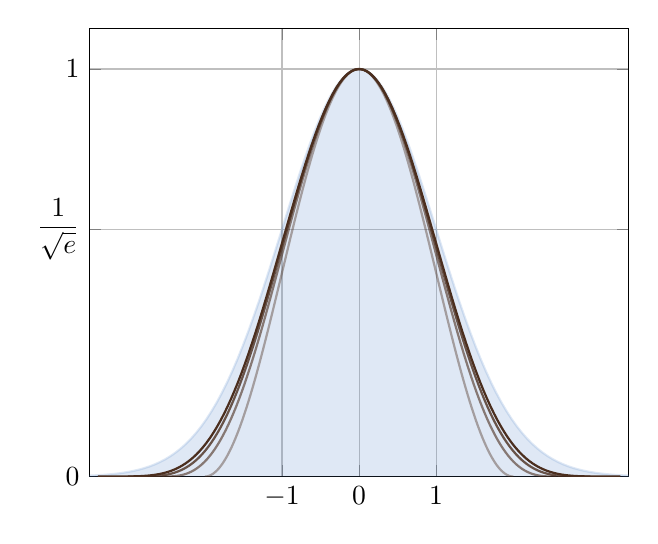
\begin{tikzpicture}[scale=1]
    \begin{axis}[
        xmin = -3.5, xmax = 3.5,
        ymin = -0.0, ymax = 1.1,
        mark=none,
        xtick={-1,0,1},
        ytick={0,{1/sqrt(e)}, 1},
        xticklabels={$-1$,$0$,$1$},
        yticklabels={$0$,$\dfrac{1}{\sqrt e}$,$1$},
        grid=major,
        minor tick num=0,
    ]
    \addplot[color=PBlue, fill=PBlue, opacity=0.2, domain=-5:5, thick, samples=150]{exp(-(x^2/2))};
    \addplot[color=PDarkBrown, opacity=0.4, domain=-2:2, thick, samples=150]{cos(x * 45)^2};
    \addplot[color=PDarkBrown, opacity=0.6, domain=-2.553:2.553, thick, samples=150]{cos(x * atan(1/sqrt(2)))^3};
    \addplot[color=PDarkBrown, opacity=0.8, domain=-3:3, thick, samples=150]{cos(x * 30)^4};
    \addplot[color=PDarkBrown, opacity=1.0, domain=-3.389:3.389, thick, samples=150]{cos(x * atan(0.5))^5};
    \end{axis}
    
\end{tikzpicture}

    \end{center}
  \end{column}
  \end{columns}
  \end{frame}

  \subsection{A Gauss fügvény integrálja}
  \begin{frame}[t]{A Gauss függvény integrálja}
  \begin{blockthm}
  \[\int_{-\infty}^{+\infty} g(x)\, dx = \sqrt{\pi}\]
  \end{blockthm}
\end{frame}

\begin{frame}[t]{}
 \begin{block}{Ez egy általános blokk}
Transzformáció:
\[G_{\mu, \sigma}(x) := g\left(\frac{x-\mu}{\sigma}\right)\]
\end{block}

\begin{alertblock}{Figyelem!}
Transzformáció:
\[G_{\mu, \sigma}(x) := g\left(\frac{x-\mu}{\sigma}\right)\]
\end{alertblock}
\end{frame}

\section{Fourier-transzformáció}

\section{A hővezetési egyenlet}
\begin{frame}[t]{A hővezetés egyenlete}
\begin{blockdef}{Hővezetési egyenlet}
\[\partial_0 u (t,x) = -D\partial^2_1 u(t,x)\] 
\end{blockdef}
\end{frame}


\section{Megoldások}

\begin{frame}[t]{}
Az a) állítás egyenesen következik az exponenciális függvény azon tulajdonságából, hogy mindig pozitív: $\exp(x)>0$.

A monotonitás vizsgálatához a függvény deriváltja: $g'(x)=-xg(x),$ és mivel $g(x)>0,$ ezért a derivált előjelét a $(-x)$
tag előjele dönti el, amiből a b) és c) állítás már adódik.
A globális maximum $g(0) = 1$ az előző két állításból következik.

Az inflexiós pontok meghatározásához a második deriváltat vizsgáljuk: $g''(x) = (x^2-1)g(x).$
A $g$ függvény a $(-\infty, -1)$ és az $(1, +\infty)$ intervallumokon 
konkáv ($g''(x)>0$), illetve a $(-1, 1)$ intervallumon konvex ($g''(x)<0$).
A $g''$ függvénynek zérushelye, és így a $g$ függvénynek inflexiós pontja van az $x=\pm1$ pontokban.
\end{frame}

\begin{frame}[t]{}
\[f''_n(x) = n\cos^{n-2}(x)\left((n-1)\sin^2(x) - cos^2(x)\right)\]
\end{frame}
\end{document}
